\documentclass{beamer}

% Font selection
\usepackage{palatino}

% Beamer template
\usetheme{Antibes}
%\usetheme{Berlin}

\usepackage[scale=1.2]{ccicons}

\usepackage[utf8]{inputenc}
\usepackage[T1]{fontenc}

\usepackage{tabularx}
\usepackage{multicol}
\usepackage{graphicx}
\usepackage[final]{pdfpages}

\usepackage{listings}

\lstset{
  language=[ISO]C++,
  columns=flexible,
  identifierstyle=\itshape,
%
  belowcaptionskip=1\baselineskip,
  breaklines=true,
  xleftmargin=\parindent,
  language=C++,
  showstringspaces=false,
  basicstyle=\small,
  keywordstyle=\bfseries\color{green!40!black},
  commentstyle=\itshape\color{purple!40!black},
  identifierstyle=\color{blue},
  stringstyle=\color{brown},
  columns=flexible,
%  inputenconding=utf8,
  extendedchars=true,
%
  morekeywords=[1]{constexpr,nullptr,alignof,alignas,decltype,noexcept,override,final,concept,expects,ensures,assert,axiom,audit},
  literate={%
    {¿}{{?`}}1
    {¡}{{!`}}1
    {á}{{\'a}}1
    {é}{{\'e}}1
    {í}{{\'i}}1
    {ó}{{\'o}}1
    {ú}{{\'u}}1
    {ñ}{{\~n}}1
}
}

\lstset{
}


\newcommand{\cppkey}[1]{%
{\color{green!40!black}\textbf{#1}}%
}

\newcommand{\cppid}[1]{%
{\color{blue}\textbf{#1}}%
}


\usepackage{tikz}
\usetikzlibrary{positioning}
\usetikzlibrary{arrows}
\usetikzlibrary{mindmap}

\usepackage{pgfplots}
\pgfplotsset{compat=1.5}


\newcommand{\textgood}[1]{%
{\color{blue}\textbf{#1}}%
}

\newcommand{\textbad}[1]{%
{\color{red}\textbf{#1}}%
}

\newcommand{\textenum}[1]{%
{\color{blue!60!black}\textbf{#1}}%
}

\newcommand{\textmark}[1]{%
{\color{orange!70!black}\textbf{#1}}%
}




% Footline in every slide
\setbeamertemplate{footline}{
  \leavevmode%
  \hbox{\begin{beamercolorbox}[wd=\paperwidth,ht=2.5ex,dp=1.125ex,leftskip=.3cm,rightskip=.3cm]{author in head/foot}%
    \usebeamerfont{author in head/foot}\ccbyncndeu 
     \quad -- \quad J. Daniel Garcia 
     -- ARCOS@UC3M (\textbf{\url{josedaniel.garcia@uc3m.es}}) 
     -- Twitter: \textbf{\url{@jdgarciauc3m}}
    \hfill
    \insertframenumber/\inserttotalframenumber
  \end{beamercolorbox}}%
  \vskip0pt%
}

% Logo in every slide
\addtobeamertemplate{headline}{}
{% 
\begin{tikzpicture}[remember picture,overlay]
\node[anchor=north east] at (current page.north east) {
\includegraphics[height=0.7cm]{logos/arcos_t.png}};
\end{tikzpicture}
}

\tikzset{
  invisible/.style={opacity=0},
  visible on/.style={alt=#1{}{invisible}},
  alt/.code args={<#1>#2#3}{%
    \alt<#1>{\pgfkeysalso{#2}}{\pgfkeysalso{#3}} % \pgfkeysalso doesn't change the path
  },
}

%Portada
\title{C++ prgramming in a parallel world}
\subtitle{CPP Europe\\Bucharest 2020}
\author{J. Daniel Garcia}
\institute{ARCOS Group\\University Carlos III of Madrid\\Spain}
\date{February 25th, 2020}

\begin{document}

\begin{frame}
\titlepage
\end{frame}

\AtBeginSection[]
{
  \begin{frame}<*>
    \setbeamertemplate{section in toc shaded}[default][50]
    \setbeamertemplate{subsection in toc shaded}[default][50]
    \tableofcontents[currentsection,hideallsubsections]
  \end{frame}
}

\AtBeginSubsection[]
{
  \begin{frame}<beamer>
    \setbeamertemplate{subsection in toc shaded}[default][50]
    \tableofcontents[sectionstyle=show/hide,subsectionstyle=show/shaded/hide]
  \end{frame}
}

\begin{frame}{Warning}

\begin{tabularx}{.98\textwidth}{lX}
\ccLogo & This work is under 
Attribution-NonCommercial-NoDerivatives 4.0 International (CC BY-NC-ND 4.0) license.\\

& You are \textbf{free} to
\textbf{Share} — copy and redistribute the material in any medium or format.
\\

\ccAttribution & 
You must give appropriate credit, provide a link to the license, and indicate if changes were made. You may do so in any reasonable manner, but not in any way that suggests the licensor endorses you or your use.\\

\ccNonCommercialEU &
You may not use the material for commercial purposes.
\\

\ccNoDerivatives &
If you remix, transform, or build upon the material, you may not distribute the modified material.
\\

\end{tabularx}

\end{frame}

\begin{frame}[t]{Who am I?}
\begin{itemize}
  \item A C++ programmer.
    \begin{itemize}
      \item Started writing C++ code in 1989.
    \end{itemize}
  \vfill\pause
  \item A university professor in Computer Architecture.
    \begin{itemize}
      \item University Carlos III of Madrid (since 2001).
    \end{itemize}
  \vfill\pause
  \item An ISO C++ language standards committee member.
    \begin{itemize}
      \item AENOR: Spanish Standards National Body.
    \end{itemize}
  \vfill\pause
  \item \textgood{My goal}: Improve applications programming.
    \begin{itemize}
      \item \textmark{Performance} $\rightarrow$ \textgood{faster} applications.
      \item \textmark{Energy efficiency} $\rightarrow$ \textgood{better} performance per Watt.
      \item \textmark{Maintainability} $\rightarrow$ \textgood{easier} to modify.
      \item \textmark{Reliability} $\rightarrow$ \textgood{safer} components.
    \end{itemize}
\end{itemize}
\end{frame}

\begin{frame}{ARCOS@uc3m}
\begin{itemize}
  \item \textbf{UC3M}: A young international research oriented university.
  \vfill
  \item \textbf{ARCOS}: An applied research group.
    \begin{itemize}
      \item \textmark{Lines}: 
            High Performance Computing,
            Big data,
            Cyberphysical systems,
            \textgood{Programming Models for Applications Improvement}.
    \end{itemize} 
  \vfill
  \item \textbf{Improving applications}:
    \begin{itemize}
      \item \textmark{REPARA}: Reengineering and Enabling Performance and poweR of Applications.
            FP7-ICT (2013--2016).
      \item \textmark{RePhrase}: REfactoring Parallel Heterogeneous Resource Aware Applications.
            H2020-ICT (2015--2018).
      \item \textmark{ASPIDE}: exAScale ProgrammIng models for extreme Data procEssing.
            H2020-FET-HPC (2018--2020).
    \end{itemize} 
  \vfill
  \item \textbf{Standardization}:
    \begin{itemize}
      \item ISO/IEC JTC/SC22/WG21. ISO C++ Committee.
    \end{itemize}
\end{itemize}
\end{frame}

\section{Times have changed}

\begin{frame}[t]{First microprocessor}
\begin{columns}[T]
  \begin{column}{.7\textwidth}
    \begin{itemize}
      \item Intel 4004 (1971).
        \begin{itemize}
          \item \textmark{Application domain}: Calculators.
          \item \textmark{Technology}: 10,000 nm.
          \vfill
          \item \textenum{Data}:
            \begin{itemize}
              \item 2300 transistors.
              \item 13 mm2
              \item 108 KHz
              \item 12 Volts
            \end{itemize}
          \vfill
          \item \textenum{Features}:
            \begin{itemize}
              \item 4-bits data.
              \item Data-path in one cycle.
            \end{itemize}
      \end{itemize}
    \end{itemize}
  \end{column}
  \begin{column}{.3\textwidth}
    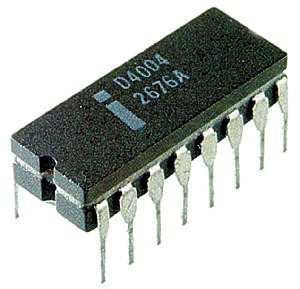
\includegraphics[width=.8\textwidth]{images/intel-4004.jpg}\\
    \begin{tiny}
      \emph{Intel 4004} photo by Rostislav Lisovy\\
    \end{tiny}
    \vspace{1em}
    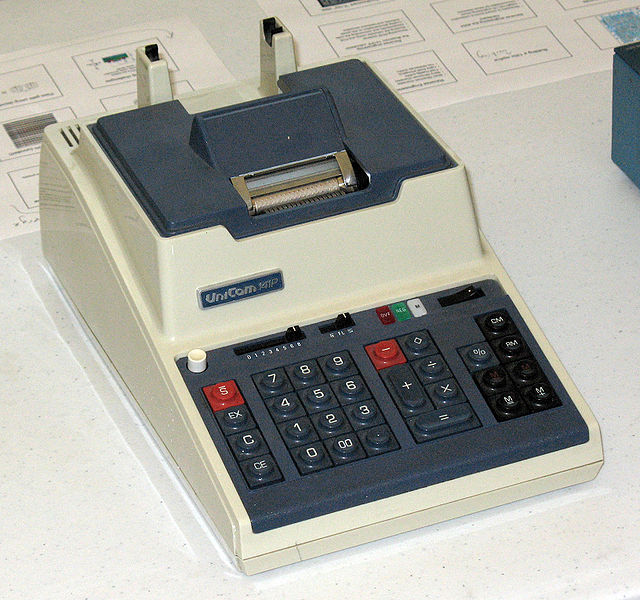
\includegraphics[width=.8\textwidth]{images/i4004-calculator.jpg}\\
    \begin{tiny}
      \emph{Unicom 141P Calculator 3} photo by Michael Holley.\\ 
    \end{tiny}
  \end{column}
\end{columns}
\end{frame}

\begin{frame}[t]{My first computer}
Sinclair ZX-Spectrum
\begin{columns}[T]
  \begin{column}{.7\textwidth}
    \begin{itemize}
      \item Zilog Z80 (1976).
        \begin{itemize}
          \item \textmark{Application domain}: Home computers, videoconsoles.
          \item \textmark{Technology}: 4,000 nm.
          \vfill
          \item \textenum{Data}:
            \begin{itemize}
              \item 8500 transistors.
              \item 2.5 MHz
              \item 5 Volts
            \end{itemize}
          \vfill
          \item \textenum{Features}:
            \begin{itemize}
              \item 8-bits data.
            \end{itemize}
      \end{itemize}
    \end{itemize}
  \end{column}
  \begin{column}{.3\textwidth}
    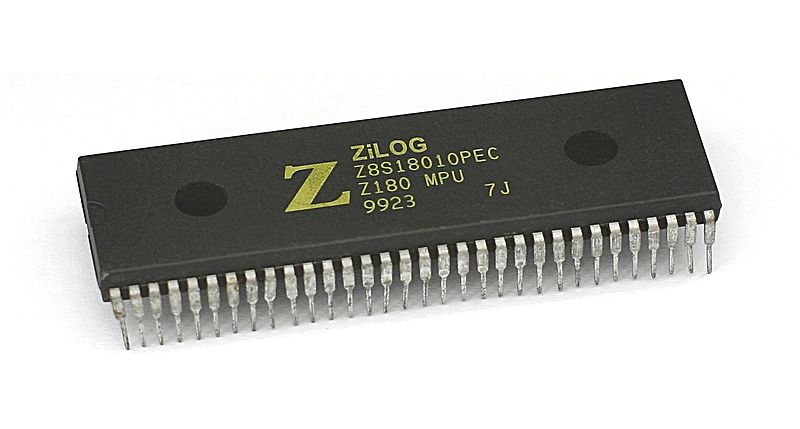
\includegraphics[width=.8\textwidth]{images/z80-micro.jpg}\\
    \begin{tiny}
      \emph{Zilog Z80} photo by Konstantin Lanzet\\
    \end{tiny}
    \vspace{1em}
    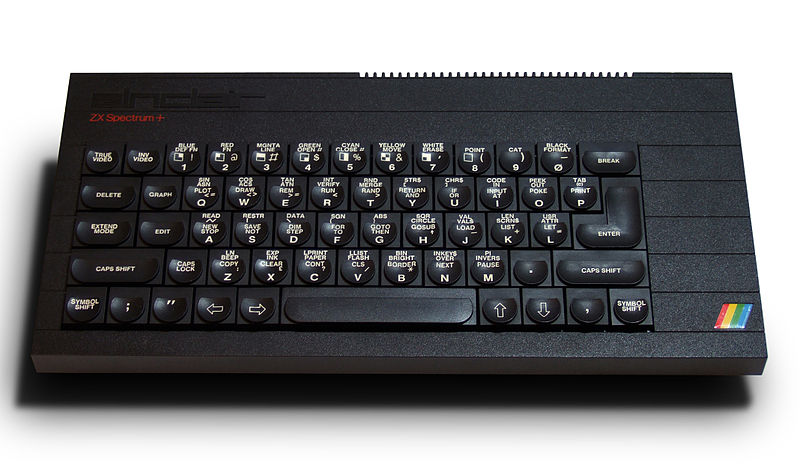
\includegraphics[width=.8\textwidth]{images/zx-spectrum.jpg}\\
    \begin{tiny}
      \emph{ZX Spectrum} photo by Bill Bertram.\\ 
    \end{tiny}
  \end{column}
\end{columns}
\end{frame}

%\begin{frame}[t]{My first PC}
%Intel 8088
%\end{frame}

\begin{frame}[t]{Last single core}
\vspace{-1em}
\begin{columns}
  \begin{column}{.15\textwidth}
    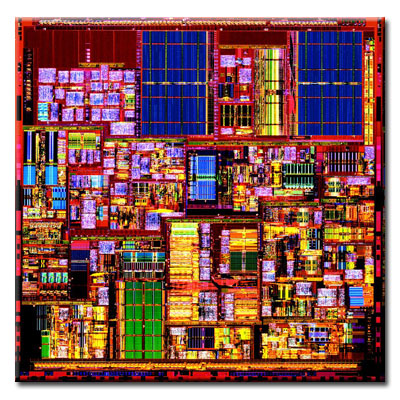
\includegraphics[width=\textwidth]{images/intel-p4-die.jpg}\\
    \begin{tiny}
      Die of Intel Pentium 4 (Northwood)\\ 
      Source: \url{http://gecko54000.free.fr}\\
    \end{tiny}
    \vspace{0.75em}
    \begin{center}
      
\includegraphics[width=.9\textwidth]{images/intel-p4.jpg}\\
    \end{center}
  \end{column}
  \begin{column}{.85\textwidth}
    \begin{itemize}
      \item Intel Pentium 4 (2003).
        \begin{itemize}
          \item \textmark{Application domain}: Desktop / Servers.
          \item \textmark{Technology}: 90 nm (1/100x).
        \end{itemize}
      \item \textenum{Data}:
        \begin{itemize}
          \item 55M transistors (20,000x).
          \item 101 mm$^2$ (10x).
          \item 3.4 GHz (10,000x).
          \item 1.2 Volts (1/10x).
        \end{itemize}
      \item \textenum{Features}:
        \begin{itemize}
          \item 32/64-bit data (16x).
          \item Data path with 22 pipeline stages (later 31).
          \item 3-4 instructions per cycle (superscalar).
          \item Two level cache on chip.
          \item Data parallel instructions (SIMD).
          \item Hyper-threading.
        \end{itemize}
    \end{itemize}
  \end{column}
\end{columns}
\end{frame}

\begin{frame}[t]{A typical multicore}
\vspace{-1em}
\begin{columns}
  \begin{column}{.7\textwidth}
    \begin{itemize}
      \item Intel Core i7 (2009).
        \begin{itemize}
          \item \textmark{Application}: Desktop / Server.
          \item \textmark{Technology}: 45 nm (1/2x).
        \end{itemize}
      \item \textenum{Data}:
        \begin{itemize}
          \item 774M transistors (12x).
          \item 296 mm$^2$ (3x).
          \item 3.2 GHz -- 3.6 GHz ($\approx$1x).
          \item 0.7 -- 1.4 Volts ($\approx$1x).
        \end{itemize}
      \item \textenum{Features}:
        \begin{itemize}
          \item 128-bit data (2x).
          \item Datapath with 14-stage pipeline (0.5x).
          \item 4 instructions per cycle ($\approx$1x).
          \item Three level cache on chip.
          \item Data parallel instructions (SIMD).
          \item 4 cores (4x) + Hyper-threading.
        \end{itemize} 
    \end{itemize}
  \end{column}
  \begin{column}{.35\textwidth}
    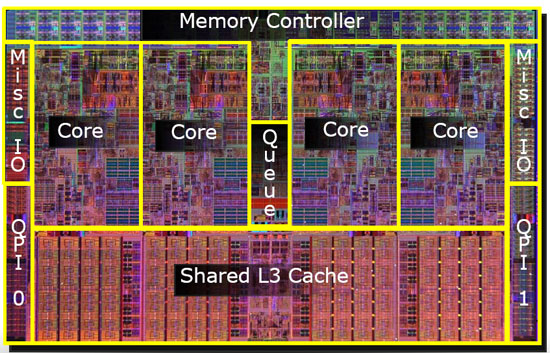
\includegraphics[width=\textwidth]{images/intel-core-i7-die.jpg}\\
    \begin{tiny}
      Die of Intel Core i7 (Nehalem)\\
      Source: \url{www.legitreviews.com}\\
    \end{tiny}
    \vspace{0.75em}
    \begin{center}
    
\includegraphics[width=.65\textwidth]{images/intel-core-i7.jpg}\\
    \end{center}
  \end{column}
\end{columns}
\end{frame}

\begin{frame}[t]{What happened?}
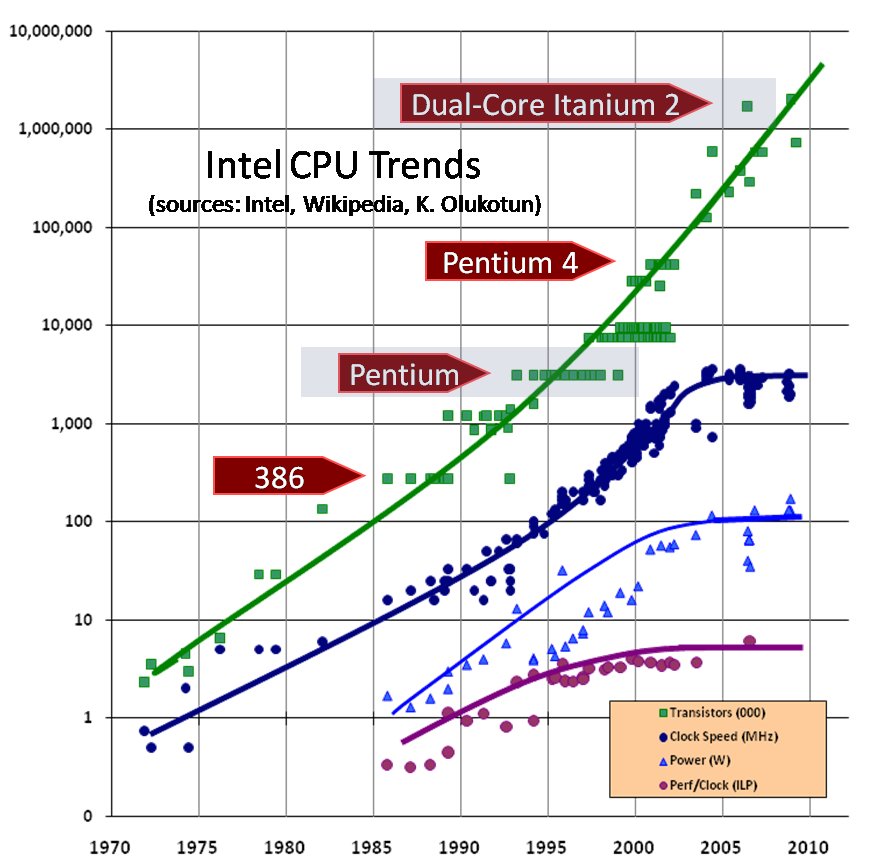
\includegraphics[height=.8\textheight,width=\textwidth]{images/free-lunch.png}\\
\begin{tiny}
Source: \alert{The free lunch is over}.
Herb Sutter.
\url{http://www.gotw.ca/publications/concurrency-ddj.htm}\\
\end{tiny}
\end{frame}

%\begin{frame}[t]{Hetorogeneity}
%\begin{itemize}
%  \item Welcome to the jungle!
%\end{itemize}
%\end{frame}

\section{What do you do with multicore?}

\begin{frame}[t]{Impact of multicores}
\begin{itemize}
\item Increase \textgood{throughput}:
  \begin{itemize}
    \item More transactions per second.
    \item Mostly \textmark{concurrent programming}.
  \end{itemize}

\item Increase performance
  \begin{itemize}
    \item Faster execution of a task.
    \item Mostly \textmark{parallel programming}.
  \end{itemize}
\end{itemize}
\end{frame}

\begin{frame}[t]{C++11/14}
\begin{itemize}
  \item Focused in providing the concurrency building blocks.
  \item Main features:
    \begin{itemize}
      \item Clear definition of the memory model.
      \item Support for TLS (\cppkey{thread\_local}).
      \item Concurrency portable abstractions:
        \begin{itemize}
          \item \cppid{std::thread}.
          \item \cppid{std::mutex}, \cppid{std::timed\_mutex}, \ldots
          \item \cppid{std::condition\_variable}, \cppid{condition\_variable\_any}.
          \item \cppid{std::unique\_lock}, \ldots
          \item \cppid{std::promise}, \cppid{std::future}, \cppid{std::packaged\_task}.
        \end{itemize}
      \item Low level portable \emph{lock-free} abstractions:
        \begin{itemize}
          \item \cppid{std::atomic}.
          \item \cppid{std::memory\_order}.
        \end{itemize}
    \end{itemize}
\end{itemize}
\end{frame}

\section{Parallelism in C++17}

\subsection{Introduction}

\begin{frame}[t,fragile]{Parallel algoritms}
\begin{itemize}
  \item Many algorithms in the STL have now
        a parallel version.
    \begin{itemize}
      \item They take a new first argument to
            specify the execution policy.
    \end{itemize}
\end{itemize}
\begin{lstlisting}[escapeinside={<@}{@>}]
// Traditional way -> sequential
std::for_each(v.begin(), v.end(), [](auto & x) { f(x); });
<@\pause @>
// New parallel
std::for_each(<@\textcolor{red}{std::execution::par}@>,
  v.begin(), v.end(), [](auto & x) { f(x); });
<@\pause @>
// New sequential
std::for_each(<@\textcolor{red}{std::execution::seq}@>,
  v.begin(), v.end(), [](auto & x) { f(x); });
\end{lstlisting}
\end{frame}

\begin{frame}[t,fragile]{Processing images}
\begin{lstlisting}
#include <vector>
#include <execution>

#include "image.h"

int main() {
  std::vector<image> v = load_images("file.dat");

  std::for_each(std::execution::par,
    v.begin(), v.end(), [](auto & img) { img.to_gray(); });

  store_images("newfile.dat", v);
}
\end{lstlisting}
\end{frame}

\begin{frame}[t,fragile]{Sorting}
\begin{itemize}
  \item Sorting requires many applications of the comparator.
    \begin{itemize}
      \item Specially interesting when comparator is not trivial.
    \end{itemize}
\end{itemize}
\begin{lstlisting}
std::vector<customer> v = get_customers();

std::sort(std::execution::par, v.begin(), v.end(),
  [](const auto & e1, const auto & e2) {
    if (e1.name == e2.name) return e1.last < e2.last;
    else return e1.name < e2.name;
  }
);
\end{lstlisting}
\end{frame}

\subsection{Execution policies}

\begin{frame}[t]{Overview of execution policies}
\vspace{-1em}
\begin{itemize}
  \item \cppid{std::execution::seq}.
    \begin{itemize}
      \item Class \cppid{std::execution::sequenced\_policy}.
      \item Algorithm executes sequentially (single thread).
      \item Might have changes over traditional algorithm.
    \end{itemize}
\pause
  \item \cppid{std::execution::par}.
    \begin{itemize}
      \item Class \cppid{std::execution::parallel\_policy}.
      \item Algorithm executes in multiple threads.
      \item No vectorization!
    \end{itemize}
\pause
  \item \cppid{std::execution::par\_unseq}.
    \begin{itemize}
      \item Class \cppid{std::execution::parallel\_unsequenced\_policy}.
      \item Algorithm executes in multiple threads.
      \item Vectorization allowed!
    \end{itemize}
\pause
  \item \cppid{std::execution::unseq} (\textbf{\textcolor{red}{C++20}}).
    \begin{itemize}
      \item Class \cppid{std::execution::unsequenced\_policy}.
      \item Algorithm executes in single thread.
      \item Vectorization allowed!
    \end{itemize}
\end{itemize}
\end{frame}

\begin{frame}[t,fragile]{Constraints on iterators}
\begin{itemize}
  \item Some algorithms on the STL require ranges expressed
        as \textmark{input iterators}.
\begin{lstlisting}
template< class InputIt, class T >
typename iterator_traits<InputIt>::difference_type
  count(InputIt first, InputIt last, const T &value );
\end{lstlisting}

  \item Execution policy based require iterators to be
        \textmark{forward iterators}
\begin{lstlisting}
template< class ExecutionPolicy, class ForwardIt, class T >
typename iterator_traits<ForwardIt>::difference_type
  count(ExecutionPolicy&& policy, 
        ForwardIt first, ForwardIt last, const T &value );
\end{lstlisting}
\end{itemize}
\end{frame}

\begin{frame}[t,fragile]{Changes in algorithms interface}
\begin{itemize}
  \item Some algorithms have changed their return types.
  \vfill\pause
  \item Without execution policy.
    \begin{itemize}
      \item Returns the comparator object.
    \end{itemize}
\begin{lstlisting}
template <class InputIt, class UnaryFunction>
constexpr UnaryFunction 
  for_each(InputIt first, InputIt last, UnaryFunction f);
\end{lstlisting}
  \vfill\pause
  \item With execution policy.
    \begin{itemize}
      \item Does not return any value.
    \end{itemize}
\begin{lstlisting}[escapeinside={<@}{@>}]
template <class ExecutionPolicy, class ForwardIt, 
          class UnaryFunction2>
<@\textcolor{red}{void}@>
  for_each(ExecutionPolicy&& policy, 
           ForwardIt first, ForwardIt last, UnaryFunction2 f);
\end{lstlisting}
\end{itemize}
\end{frame}

\begin{frame}[t,fragile]{What about exceptions?}
\begin{itemize}
  \item In non execution policy based exceptions can be thrown.
\begin{lstlisting}
std::for_each(v.begin(), v.end(),
  [](auto & x) {
    if (valid(x)} f(x);
    else throw invalid_value{x}; // Throws exception
  });
\end{lstlisting}

\vfill\pause
  \item In excecution policy based exceptions translate into 
        \cppid{std::terminate}.

\begin{lstlisting}
std::for_each(std::execution::seq, v.begin(), v.end(),
  [](auto & x) {
    if (valid(x)} f(x);
    else throw invalid_value{x}; // Invoke std::terminate
  });
\end{lstlisting}
\end{itemize}
\end{frame}

\begin{frame}[t]{When to avoid execution policies}
\begin{itemize}
  \item Using input or output iterators.
  \vfill\pause
  \item Avoid calling \cppid{std::terminate} on exceptions.
  \vfill\pause
  \item Avoid side effects on use of elements.
  \vfill\pause
  \item Make use of return values (e.g. \cppid{std::for\_each()}.
\end{itemize}
\end{frame}

\subsection{Updating global state}

\begin{frame}[t,fragile]{Counting valid elements}
\begin{lstlisting}
long count = 0;
std::vector<double> v = get_values();

std::for_each(std::execution::par,
  v.begin(), v.end(),
  [](double x) {
    if (x>0) count++;
  }
);

std::cout << "Count= " << count << "\n";
\end{lstlisting}
\end{frame}

\begin{frame}[t,fragile]{Solving the data race: mutexes}
\begin{lstlisting}
long count = 0;
std::mutex m;
std::vector<double> v = get_values();

std::for_each(std::execution::par,
  v.begin(), v.end(),
  [](double x) {
    if (x>0) {
      std::lock_guard<std::mutex> l{m};
      count++;
    }
  }
);

std::cout << "Count= " << count << "\n";
\end{lstlisting}
\end{frame}

\begin{frame}[t,fragile]{Solving the data race: atomics}
\begin{lstlisting}
std::atomic<long> count = 0;
std::vector<double> v = get_values();

std::for_each(std::execution::par,
  v.begin(), v.end(),
  [](double x) {
    if (x>0) count++;
  }
);

std::cout << "Count= " << count << "\n";
\end{lstlisting}
\end{frame}

\begin{frame}[t,fragile]{Or even better}
\begin{lstlisting}
std::vector<double> v = get_values();

long count = std::count_if(std::execution::par,
  v.begin(), v.end(),
  [](double x) {
    return x>0
  }
);

std::cout << "Count= " << count << "\n";
\end{lstlisting}
\end{frame}

\begin{frame}[t]{Remember}
\begin{itemize}
  \item Accessing global state from algorithms may result
        in data races.
    \begin{itemize}
      \item Using mutexes may be a heavyweight solution.
      \item Atomics hav limited applicability.
    \end{itemize}

  \vspace{1em}\pause
  \item There might be a better algorithm.
    \begin{itemize}
      \item A \cppid{std::for\_each()} call may be
            a \textmark{code smell}.
    \end{itemize}
\end{itemize}
\end{frame}


\subsection{Transformations}

\begin{frame}[t]{The map-pattern}
\begin{itemize}
  \item A well known pattern in functional programming.
    \begin{itemize}
      \item Apply an operation to every element in a data set
            to generate a new data set.
    \end{itemize}
\end{itemize}
\end{frame}

\begin{frame}[t,fragile]{Squaring values}
\begin{lstlisting}
std::vector<double> square(const std::vector<double> & v) 
{
  std::vector<double> r(v.size());

  std::transform(std::sequential::par,
    v.begin(), v.end(), r.begin(),
    [](double x) { return x*x; }
  );

  return r;
}
\end{lstlisting}
\end{frame}

\begin{frame}[t,fragile]{Adding vectors}
\begin{lstlisting}
std::vector<double> add(const std::vector<double> & v,
                           const std::vector<double> & w) 
{
  std::vector<double> r(v.size());

  std::transform(std::sequential::par,
    v.begin(), v.end(), w.begin(), r.begin(),
    [](double x, double y) { return x+y; }
  );

  return r;
}
\end{lstlisting}
\end{frame}

\begin{frame}[t,fragile]{Heterogeneous transformations}
\begin{lstlisting}
std::vector<std::complex<double>> create_cplx(
    const std::vector<double> & re,
    const std::vector<double> & im)
{
  auto sz = std::min(re.size(), im.size());
  std::vector<std::complex<double>> res(sz);
  
  std::transform(std::execution::par,
    re.begin(), re.end(), im.begin(),
    res.begin(),
    [](double r, double i) -> complex<double> {
      return {r,i};
    });
  return res;
}
\end{lstlisting}
\end{frame}

\subsection{Reductions}

\begin{frame}[t]{Reduction pattern}
\begin{itemize}
  \item A \textmark{reduction} computes the sum of all elements
        in a data set.

  \vspace{1em}\pause
  \item \textbad{Note}: \cppid{std::reduce} looks quite similar
        to \cppid{std::accumulate} on the surface.
    \begin{itemize}
      \item Result is not deterministic unless the sum opration
            is both associative and commutative.
    \end{itemize}
\end{itemize}
\end{frame}

\begin{frame}[t,fragile]{Add all elements in a vector}
\begin{lstlisting}
void print_add(const std::vector<double> & v)
{
  double r = std::reduce(std::execution::par,
    v.begin(), v.end());

  std::cout << "sum= " << r << "\n";
}
\end{lstlisting}
\vfill
\begin{itemize}
  \item Initial value is \cppid{value\_type\{\}}.
  \item Binary operation is \cppid{std::plus<>()}.
\end{itemize}
\end{frame}

\begin{frame}[t,fragile]{Providing initial value}
\begin{lstlisting}
void print_add(const std::vector<double> & v)
{
  double r = std::reduce(std::execution::par,
    v.begin(), v.end(), 100.0);

  std::cout << "sum= " << r << "\n";
}
\end{lstlisting}
\begin{itemize}
  \item Still reduction operation is \cppid{std::plus<>()}.
\end{itemize}
\end{frame}

\begin{frame}[t,fragile]{Providing reduction operator}
\begin{lstlisting}
void print_add(const std::vector<double> & v)
{
  double r = std::reduce(std::execution::par,
    v.begin(), v.end(), 0.0,
    [](double x, double y) { return x+y; }
  );

  std::cout << "sum= " << r << "\n";
}
\end{lstlisting}
\end{frame}


\subsection{Map/Reduce}

\begin{frame}[t]{Map/reduce pattern}
\begin{itemize}
  \item A \textmark{map-reduce} pattern combines a 
        \textgood{map} pattern with a \textgood{reduce} pattern
        over the results of that map.
    \begin{itemize}
      \item In C++ it is spelled out \cppid{std::transform\_reduce}.
    \end{itemize}
\end{itemize}
\end{frame}

\begin{frame}[t,fragile]{Computing the norm of a vector}
\begin{lstlisting}
void print_norm(const std::vector<double> & v)
{
  double s = std::transform_reduce(std::execution::par,
    v.begin(), v.end(),
    0.0,
    [](double x, double y) { return x + y },
    [](double x) { return x * x; }
  );

  std::cout << "Norm: " << std::sqrt(s) << "\n";
}
\end{lstlisting}
\end{frame}

\begin{frame}[t,fragile]{Computing aggregate area}
\begin{lstlisting}
double area(const std::vector<shape> & shapes)
{
  return std::map_reduce(std::execution::par,
    shapes.begin(), shapes.end(),
    0.0,
    [](double x, double y) { return x+y; },
    [](const shape & s) { return s.area(); }
  );
}
\end{lstlisting}
\end{frame}

\begin{frame}[t,fragile]{Cannonical example}
\begin{itemize}
  \item Word frequencies from sequence of words.
    \begin{itemize}
      \item Associative container with \cppid{<word,freq>}.
    \end{itemize}
\end{itemize}
\begin{lstlisting}[escapeinside={<@}{@>}]
auto word_freq(const std::vector<std::string> & words) 
{<@\pause{}@>
  using dictionary = std::map<std::string,long>;<@\pause{}@>
  return std::transform_reduce(std::execution::par,<@\pause{}@>
    words.begin(), words.end(), dictionary{},<@\pause{}@>
    [](dictionary & lhs, const dictionary & rhs) -> dictionary {
      for (auto & [key,value] : rhs) { lhs[key] += value; }
      return lhs;
    },<@\pause{}@>
    [](const std::string & s) -> dictionary { return {w,1}; }
  );
}
\end{lstlisting}
\end{frame}

\subsection{Scans}

\begin{frame}[t]{Scan pattern}
\begin{itemize}
  \item A \textmark{scan} pattern computes a sequence of
        partial reductions on a dataset.
    \begin{itemize}
      \item A scan on $x_0$, $x_1$, $x_2$, \ldots 
      \item Results in the sequence:
        \begin{itemize}
          \item $x_0$
          \item $x_0 + x_1$
          \item $x_0 + x_1 + x_2$
          \item \ldots
        \end{itemize}
    \end{itemize}
    \vfill
    \item Two alternatives:
      \begin{itemize}
        \item \cppid{std::exclusive\_scan()}
        \item \cppid{std::inclusive\_scan()}
      \end{itemize}
\end{itemize}
\end{frame}

\begin{frame}[t,fragile]{Computing CDF}
\begin{lstlisting}
auto compute_cdf(const std::vector<int> & histogram)
{
  std::vector<int> cdf(histogram.size());

  std::inclusive_scan(std::execution::par,
    histogram.begin(), histogram.end(),
    cdf.begin(),
    0
  );

  return cdf;
}
\end{lstlisting}
\end{frame}

\begin{frame}[t,fragile]{Combining transform and scan}
\begin{lstlisting}
auto compute_cdf(const std::vector<int> & histogram)
{
  std::vector<int> cdf(histogram.size());

  std::transform_inclusive_scan(std::execution::par,
    histogram.begin(), histogram.end(),
    cdf.begin(),
    0,
    [](auto x, auto y) { return x+y; }
    [](auto x) {
      if (x<0) return 0;
      if (x>255) return 255;
      return x;
    }
  );

  return cdf;
}
\end{lstlisting}
\end{frame}

\subsection{More algorithms}

\begin{frame}[t]{What algorithms are parallel}
\begin{itemize}
  \item Most algorithms have an execution policy based version.
  \item Few exceptions:
    \begin{itemize}
      \item Numerics replaced by new versions: 
            \cppid{accumulate}, \cppid{inner\_product},
            \cppid{partial\_sum}.
      \item Backwards algorithms:
            \cppid{copy\_backward}, \cppid{move\_backward}.
      \item Searching: some versions of \cppid{search}.
      \item Sampling and permuting:
            \cppid{sample}, \cppid{shuffle}, \cppid{*\_permutation}.
      \item Partitioning: \cppid{partition\_point}.
      \item Bounds search: \cppid{*\_bound}, \cppid{equal\_range}.
      \item Heap based: \cppid{*\_heap}.
    \end{itemize}
\end{itemize}
\end{frame}


\section{After C++20: Executors}

\begin{frame}[t]{DISCLAIMER}
\begin{quote}
This section contains tentative design that
has currently under discussion.
\end{quote}
\end{frame}

\begin{frame}[t]{Context}
\begin{itemize}
  \item A possible \textmark{future}:
    \begin{itemize}
      \item Composition of networked, asynchronous parallel computations.
      \item Accelerated by diverse hardware
    \end{itemize}
\vfill\pause
  \item But the \textmark{present}:
    \begin{itemize}
      \item Low-level concurrency primitives 
            (\cppid{std::thread}, \cppid{std::atomic}, \ldots).
      \item Components with known problems
            (\cppid{std::async}, \cppid{std::future}, \ldots).
      \item Parallel algorithms neither flexible nor composable.
    \end{itemize}
\vfill\pause
  \item \textgood{Solution} with two components:
    \begin{itemize}
      \item \cppid{executor}s
      \item \cppid{sender}s and \cppid{receiver}s.
    \end{itemize}
\end{itemize}
\end{frame}

\begin{frame}[t,fragile]{Executors}
\begin{itemize}
  \item Executors:
    \begin{itemize}
      \item A work execution interface.
        \begin{itemize}
          \item Any \cppid{executor} type.
        \end{itemize}
\begin{lstlisting}
using namespace std::execution;
std::static_thread_pool p(16);
executor auto ex = p.executor();
execute(ex, []{ do_the_work(); });
\end{lstlisting}
    \end{itemize}
\end{itemize}
\end{frame}

\begin{frame}[t,fragile]{Senders and receivers}
\begin{itemize}
  \item Senders and receivers:
    \begin{itemize}
      \item A representation of work and interrelationships.
        \begin{itemize}
          \item \cppid{sender} types.
          \item \cppid{receiver} types.
        \end{itemize}
\begin{lstlisting}
sender auto begin = schedule(ex);
sender auto next = then(begin, [] { f(); return 42; });
sender auto job = then(next, [](int x) { g(x); return 99; });

receiver auto doit = as_receier([](int x) { store(x); });
submit(job,doit);
\end{lstlisting}
    \end{itemize}
\end{itemize}
\end{frame}

\begin{frame}[t]{What is an executor}
\begin{itemize}
  \item A lightweight handle to an execution context.
    \begin{itemize}
      \item A thread pool.
      \item SIMD units.
      \item GPUs.
      \item Current thread.
      \item \ldots
    \end{itemize}
\end{itemize}
\end{frame}

\begin{frame}[t,fragile]{The simplest executor}
\begin{itemize}
  \item An inline executor executes the work immediately.
\end{itemize}
\begin{lstlisting}
struct inline_executor {
  template<class F>
  void execute(F&& f) const noexcept {
    std::invoke(std::forward<F>(f));
  }

  auto operator<=>(const inline_executor&) const = default;
};
\end{lstlisting}
\end{frame}

\begin{frame}[t,fragile]{Bulk execution}
\begin{itemize}
\item Another example of control structure provided by
      an executor.
  \begin{itemize}
    \item Creates a group of functions calls in a single operation.
  \end{itemize}
\end{itemize}
\begin{lstlisting}
struct simd_executor : inline_executor { 
  template<class F>
  simd_sender bulk_execute(F f, size_t n) const {
    #pragma simd
    for(size_t i = 0; i != n; ++i) {
      std::invoke(f, i);
    }

    return {};
  }
};
\end{lstlisting}
\end{frame}

\begin{frame}[t,fragile]{An executor based for-each}
\begin{lstlisting}
template<class Executor, class F, class Range>
void my_for_each(const Executor& ex, F f, Range rng) {
  // request bulk execution, receive a sender
  sender auto s = execution::bulk_execute(ex, 
    [=](size_t i) {
      f(rng[i]);
    }
  );

  // initiate execution and wait for it to complete
  execution::sync_wait(s);
}
\end{lstlisting}
\end{frame}

\begin{frame}[t,fragile]{A future asynchronous STL?}
\begin{lstlisting}
sender auto s = 
  just(3) |                            // produce '3' immediately
  via(scheduler1) |                    // transition context
  then([](int a){return a+1;}) |       // chain continuation
  then([](int a){return a*2;}) |       // chain another continuation
  via(scheduler2) |                    // transition context
  handle_error([](auto e){
    return just(3);});                 // with default value on errors

int r = sync_wait(s);                  // wait for the result
\end{lstlisting}
\end{frame}

\section{What can else can I do?}

\begin{frame}[t]{GrPPI}
\begin{Large}
\textgood{\url{https://github.com/arcosuc3m/grppi}}
\end{Large}
\vfill\pause
\begin{itemize}
  \item \textgood{G}eneric \textgood{r}eusable \textgood{P}arallel
        \textgood{P}attern \textgood{Interface}.
    \begin{itemize}
      \item A header only library.
      \item A set of execution policies.
      \item A set of type safe generic algorithms.
      \item Requires \textgood{C++14}.
      \item Apache 2.0 License.
    \end{itemize}
\end{itemize}
\end{frame}

\subsection{Controlling execution}

\begin{frame}[t]{Execution types}
\begin{itemize}
  \item Execution model is encapsulated in execution types.
    \begin{itemize}
      \item Always provided as first argument to patterns.
    \end{itemize}

  \vfill
  \item Current concrete execution types:
    \begin{itemize}
      \item \textmark{Sequential}: \cppid{sequential\_execution}.
      \item \textmark{ISO C++ Threads}: \cppid{parallel\_execution\_native}.
      \item \textmark{OpenMP}: \cppid{parallel\_execution\_omp}.
      \item \textmark{Intel TBB}: \cppid{parallel\_execution\_tbb}.
      \item \textmark{FastFlow}: \cppid{parallel\_execution\_ff}.
    \end{itemize}

  \vfill
  \item Run-time polymorphic wrapper through type erasure:
    \begin{itemize}
      \item \cppid{dynamic\_execution}.
    \end{itemize}
\end{itemize}
\end{frame}

\begin{frame}[t,fragile]{Execution model properties}
\begin{itemize}
  \item Some execution types allow finer configurtion.
    \begin{itemize}
      \item Example: Concurrency degree.
    \end{itemize}

  \vfill\pause
  \item Interface:
\begin{lstlisting}[basicstyle=\small]
ex.set_concurrency_degree(4);
int n = ex.concurrency_degree();
\end{lstlisting}

  \vfill\pause
  \item \textenum{Default values}:
    \begin{itemize}
      \item \textmark{Sequential} $\Rightarrow$ \cppid{1}.
      \item \textmark{Native} $\Rightarrow$ \cppid{std::thread::hardware\_concurrency()}.
      \item \textmark{OpenMP} $\Rightarrow$ \cppid{omp\_get\_num\_threads()}.
    \end{itemize}

\end{itemize}
\end{frame}


\input{pipeline}
\input{farm}
\input{stream-execution}
\input{filter}


\section{Summary}

\begin{frame}[t]{Summary}
\begin{itemize}
\item We live in a parallel world!
\vfill\pause
\item Many portable concurrency primitives since C++11.
  \begin{itemize}
    \item Low level and good for solving the througput challenge.
  \end{itemize}
\vfill\pause
\item C++17 brings easy parallelism to the STL.
  \begin{itemize}
    \item Mostly data parallelism.
   \end{itemize}
\vfill\pause
\item C++23 (hopefully) might bring executors.
\vfill\pause
\item Stream parallelism still to be solved.
\end{itemize}
\end{frame}



\begin{frame}
\titlepage
\end{frame}

\end{document}
